\documentclass[11pt,a4paper]{article}

\usepackage[utf8]{inputenc}
\usepackage[francais]{babel}
\usepackage[T1]{fontenc}
\usepackage{amsmath}
\usepackage{amsfonts}
\usepackage{amssymb}
\usepackage[colorlinks=false]{hyperref} % liens dans le sommaire
% \usepackage[top = 2.54cm, bottom = 2.54cm, left = 2.54cm, right = 2.54cm]{geometry}
\usepackage[top = 2cm, bottom = 2cm, left = 2cm, right = 2cm]{geometry}
\usepackage{graphicx}
\usepackage{caption}
\hypersetup{colorlinks, linkcolor = black, citecolor = black} % enlève couleur des liens
\usepackage{hyperref}
\usepackage{color}
\frenchbsetup{StandardLists=true}
\usepackage{float}
\usepackage{fancyhdr}
\usepackage{mathtools}
\pagestyle{fancy}

\newcommand{\dx}[1]{\dfrac{\partial #1}{\partial x}}
\newcommand{\norm}[1]{\big|\big|#1\big|\big|}
\newcommand{\question}[2]{\paragraph{Question #1 --}\hspace{-7pt}\textit{#2} \\}
\newcommand{\tphi}{\widetilde{\Phi}}
\newcommand{\intsigma}{\widetilde{\Sigma}}
\newcommand{\F}{\mathcal{F}}
\begin{document}

\begin{titlepage}
  ~\vspace{90pt}
  \centering \bfseries

  \huge Rapport de TP \\AMS302

  \vspace{50pt}
  \rule{0.5\textwidth}{1pt}
  \vspace{50pt}

  \Huge Solveur Monte-Carlo \\ pour le transport de particules neutres

  \vspace{50pt}
  \rule{0.5\textwidth}{1pt}

  \vspace{50pt}
  \huge {\itshape Benoît Sohet \\ \& \\ Aurélien Valade}

  \vfill
  \begin{tabular}{cc}
    \begin{minipage}{.49\textwidth}
      \centering
      \includegraphics[height=0.1\textheight]{logo_ups}
    \end{minipage}
    &
      \begin{minipage}{.49\textwidth}
        \centering
        \includegraphics[height=0.1\textheight]{logo_ensta}
      \end{minipage}
  \end{tabular}

\end{titlepage}

\newpage

\section{Introduction}

Dans ce TP on cherche à résoudre le problème différentiel suivant 
\begin{equation}
  \label{eq:principal}
  \begin{cases}
    \mu \dx{\Phi}(x, \mu) + \Sigma_t \Phi(x, \mu) =
    \dfrac{1}{2} \Sigma_s(x) \int_1^{-1} \Phi(x, \mu') d\mu' + S(x, \mu) & \forall (x, \mu) \in [0,1]\times[-1,1]  \medskip\\ 
    \mu n(x) < 0  & \forall (x, \mu) \in \{0,1\}\times[-1,1] 
  \end{cases}
\end{equation}

\begin{itemize}
\item $\Phi(x, \mu)$ le flux neutronique
\item $\Sigma_t$ la section efficace totale 
\item $n(x)$ la normale sortante : $n(0) = -1, ~ n(1) = 1$
\end{itemize}

On fixe pour cela deux types de conditions aux limites 
\begin{itemize}
\item Flux entrant à gauche
  \begin{equation}
    \begin{cases}
      \Phi^{-} (0, \mu) = \frac{1}{\mu}  ~~~ \forall \mu \in [0,1]\\
      \Phi^{-} (1, \mu) = 0 ~~~ \forall \mu \in [-1,0]
    \end{cases}
  \end{equation}
\item Source nulle ou unitaire
  \begin{align}
    S(x) &= 0 ~~~ \forall x \in [0,1] \\
    S(x) &= 1 ~~~ \forall x \in [0,1] 
  \end{align}
\end{itemize}	

On utilisera dans la suite l'erreur pour une fonction $f$ et son approximation $\tilde{f}$ : 
\begin{equation}
  e_{L^2}(f, \tilde{f}) = \frac{\norm{f-\tilde{f}}_{L_2}}{\norm{f}_{L_2}}
\end{equation}

\emph{L'utilisation des codes nécessite gnuplot ainsi qu'un système d'exploitation respectant la norme POSIX.}

\question{1}{Quelle est la densité de probabilité du libre parcours d'un neutron dans un matériau de section
  efficace totale $\Sigma$ ? Comment échantillonner une variable aléatoire suivant cette loi ?}
\subparagraph{Densité \textit{p} :} Nous allons d'abord calculer la fonction de répartition correspondant :
\begin{equation}
  F(l)=\int_a^{a+l} p(x) dx ,
\end{equation}
(avec $a$ une constante quelconque), puis on déduira :
\begin{equation}
  p(l)=\left\|\frac{\partial F}{\partial l}\left(l\right)\right\| .
\end{equation}

$F(l)$ est la probabilité qu'un neutron n'ait pas intéragi (ni absorption ni diffusion) lors d'un parcours de longueur $l$ selon l'axe $(0x)$, autrement dit la probabilité que ce neutron ait un libre parcours de longueur $\frac{l}{\mu}$.

Or, la probabilité qu'il n'y ait pas d'intéraction sur une longueur infinitésimal $\delta l$ est :
\begin{equation}
  1- \frac{\Sigma_t}{\mu} \delta l .
\end{equation}

Il suffit alors de multiplier cette expression autant de fois qu'il y a $\delta l$ dans $l$, c'est-à-dire $N=\frac{l}{\delta l}$, pour parvenir à $F(l)$, puisqu'on peut considérer ces évènements comme indépendants : 
\begin{equation}
  \left(1-\frac{\Sigma_t}{\mu} \delta l\right)^N = \left(1-\frac{\Sigma_t}{\mu} \frac{l}{N}\right)^N  \xrightarrow[N \rightarrow \infty]{} e^{-\frac{\Sigma_t}{\mu} l} .
\end{equation}

De là, la probabilité $p(l) dl$ d'interaction entre $l$ et $l+dl$ (sachant qu'il n'y en a pas eu jusqu'à présent) vaut :

\begin{equation}
  p(l) dl = \frac{\Sigma_t}{\mu} e^{-\frac{\Sigma_t}{\mu} l} dl .
\end{equation}

\subparagraph{Échantillonnage :}

Pour reproduire cette densité de probabilité numériquement par une variable aléatoire $X$, il suffit d'expliciter $F^{-1}$, car :
\begin{equation}
  P(a\leq X\leq b) {\color{red}=} F(b) - F(a) {\color{red}=} P(F(a)\leq U\leq F(b)) {\color{red}=} P(a\leq F^{-1}(U)\leq b) ,
\end{equation}

où $U$ est une variable aléatoire uniforme. Or :

\begin{equation}
  F^{-1}(y) = -\frac{\mu}{\Sigma_t} \log(y) .
\end{equation}

Il suffit donc d'utiliser une fonction \textit{random} numérique à valeurs dans l'image de la fonction de répartition $F$, $[0;1]$, puis d'appliquer l'inverse de cette fonction, $F^{-1}$.
On obtient ainsi la variable aléatoire suivant la loi $p(l) dl$.

\subparagraph{Remarque :} Lorsque $\mu<0$, $dl<0$ et $N<0$, mais dans chaque formule se fait le produit (ou le rapport) de deux de ces quantités, ce qui redevient alors positif.

\question{2}{Connaissant les trajectoires (marches aléatoires) d'une population neutronique, comment construire un estimateur du flux neutronique?}

Le flux neutronique en $x$ d'une population de neutrons est par définition le nombre de ces neutrons dont la trajectoire s'est arrêtée en $x$ (c'est-à-dire lorsqu'il y a eu interaction).

\section{Matériau purement absorbant}

\subsection{Matériau homogène - source ponctuelle}

\question{3}{Trouver la solution analytique au problème \autoref{eq:principal} avec les conditions suivantes :}

\begin{equation}
  \Sigma_s=0, ~~~ \dx{\Sigma_t} = 0, ~~~ S(x, \mu) = \delta(x)
\end{equation}
On a donc 
\begin{equation}
  \dx{\Phi} + \frac{\Sigma_t}{\mu} \Phi = \frac{1}{\mu} \delta(x)
\end{equation}

Une fois soumis à la transformée de Fourrier on a 
\begin{align}
  &i \omega \tphi + \frac{\Sigma_t}{\mu} \tphi = \frac{1}{\mu} \\
  &\tphi = -\frac{i}{\mu\left(\omega - \frac{i \Sigma_t}{\mu}\right)}
\end{align}
on peut donc écrire 
\begin{equation}
  \Phi (x, \mu) = -\frac{i}{2\pi\mu} \int_{\mathbb{R}} \frac{e^{i\omega x}}{\omega - \frac{i \Sigma_t}{\mu}} d\omega 
\end{equation}
or d'après le théorème des résidus appliqué sur le contour fermé autour du point singulier $\omega = i\frac{\Sigma_t}{\mu}$
\begin{equation}
  \gamma_r = [-r,r]\cup\left\{r e^{-i \theta}, \theta \in [0, \pi] \right\} ~~~ \mbox{avec } r \to \infty
\end{equation}
on trouve que
\begin{align}
  \Phi (x, \mu) &= - (2 \pi i) \frac{i}{2\pi\mu} e^{i \frac{i \Sigma_t}{\mu} x} \\
                &= \frac{1}{\mu} e^{-\frac{\Sigma_t}{\mu} x} 
\end{align}

Ces fonctions sont représentés dans la \autoref{fig:delta_many_mu}.

\begin{figure}
  \centering
  \includegraphics[height=.4\textheight]{phi_source_delta_many_mu}
  \caption{Fonctions $\Phi$ pour différent $\mu$.}
  \label{fig:delta_many_mu}
\end{figure}

\question{4-6}{Implémenter le code Monte-Carlo pour ce modèle}

Cf code commenté.

\begin{figure}
  \centering
  \includegraphics[height=0.3\textheight]{phi_sigma_cst_source_delta}
  \includegraphics[height=0.3\textheight]{phi_sigma_cst_source_cste}
  \includegraphics[height=0.3\textheight]{phi_sigma_cst_source_cste_mu_neg}
  \caption{Courbes théoriques et résultats des simuluations Monte Carlo pour différents cas de figure.
    \textbf{Haut} : source ponctuelle en 0 avec $\mu=0.5$ et $\Sigma_t=2$ pour $10^6$ particules avec une erreur $e_{L_2} = 3\,10^{-6}$. 18260 particules sont sorties du segment unitaire par la droite. 
    \textbf{Milieu} : source constante sur $[0,1]$ avec $\mu=0.5$ et $\Sigma_t=3$ pour $10^6$ particules avec une erreur $e_{L_2} = 3\,10^{-6}$.
    \textbf{Bas} :  source constante sur $[0,1]$ avec $\mu=-0.5$ et $\Sigma_t=3$ pour $10^6$ particules avec une erreur $e_{L_2} = 3\,10^{-6}$.}
  \label{fig:sigmacst}
\end{figure}

\subsection{Matériau homogène - source uniforme}

\question{5}{Trouver la solution analytique au problème \autoref{eq:principal} avec les conditions suivantes :}

\begin{equation}
  \Sigma_s=0, ~~~ \dx{\Sigma_t} = 0, ~~~ S(x, \mu) = 1
\end{equation}
On a donc en considérant un flux entrant nul à gauche 
\begin{gather}
  \dx{\Phi} + \frac{\Sigma_t}{\mu} \Phi = \frac{1}{\mu} \\
  \begin{cases}
    \Phi(x, \mu)= \frac{1}{\Sigma_t}\left( 1-e^{-\frac{\Sigma_t}{\mu}x}\right) &~~~ \mbox{si } \mu>0 \medskip \\ %\frac{1}{\mu}e^{-\frac{\Sigma_t}{\mu}x} +
    \Phi(x, \mu)= \frac{1}{\Sigma_t}\left( 1-e^{-\frac{\Sigma_t}{\mu}(x-1)}\right) &~~~ \mbox{si } \mu<0 
  \end{cases}
\end{gather}

Ces résultats sont visibles en \autoref{fig:cste_many_mu}, et les résultats des Monte-Carlo sont rassemblés en \autoref{fig:sigmacst}.
\begin{figure}
  \centering
  \includegraphics[height=.4\textheight]{phi_source_cste_many_mu}
  \caption{Fonctions $\Phi$ pour différent $\mu$.}
  \label{fig:cste_many_mu}
\end{figure}

\subsection{Matériau hétérogène - source ponctuelle}

\question{6}{Trouver la solution analytique au problème \autoref{eq:principal} avec les conditions suivantes :}

\begin{equation}
  \Sigma_s=0, ~~~
  \Sigma_t =
  \begin{cases}
    1 &\mbox{si } x<0.3 \\
    3 &\mbox{si } 0.3<x<0.7 \\
    1 &\mbox{si } 0.7<x \\
  \end{cases}
  , ~~~ S(x, \mu) = \delta(x)
\end{equation}

On pose l'intégrale continue de $\Sigma_t(x)$ 
\begin{equation}
  \intsigma(x) =
  \begin{cases}
    x &\mbox{si } x<0.3 \\
    3(x-0.3)+0.3 &\mbox{si } 0.3<x<0.7 \\
    (x-0.7)+1.5 &\mbox{si } 0.7<x \\
  \end{cases}
\end{equation}

On résout sur l'intervale $x\in[0,0.3]$ comme dans la question 3 :
\begin{equation}
  \Phi(x, \mu) = \frac{1}{\mu} e^{-\frac{\Sigma_t x)}{\mu}} ~~~ \mbox{si } x<0.3
\end{equation}
et on prolonge sur tout le segment grâce à $\intsigma(x)$ 
\begin{equation}
  \Phi(x, \mu) = \frac{1}{\mu} e^{-\frac{\intsigma(x)}{\mu}} 
\end{equation}
que l'on peut voir représentée en \autoref{fig:phi}.

\begin{figure}
  \centering
  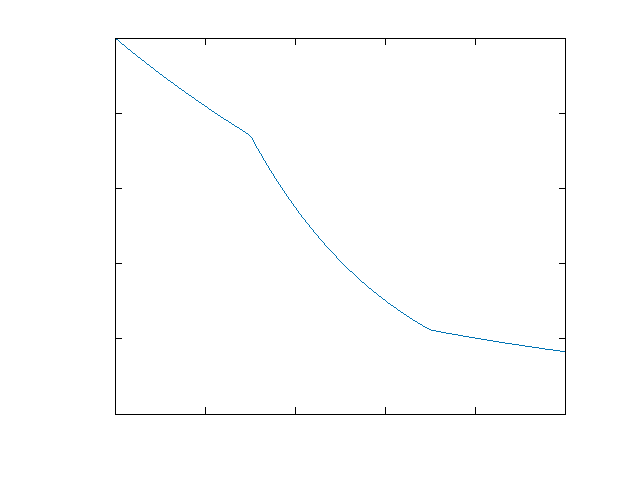
\includegraphics[width=.7\textwidth]{phi}
  \caption{Fonction $\Phi(x, \mu=1)$ pour $\Sigma_t$ variable avec une source ponctuelle en 0.}
  \label{fig:phi}
\end{figure}


\textbf{Attention : } ce raisonnement ne fonctionne que pour des particules partant de $x=0$ ! La loi de probabilité d'aller à une distance $x$ a une toute autre forme si la source est quelconque.

\question{7}{Implémenter un solveur Monte-Carlo utilisant la méthode de Woodcock pour échantillonner le libre parcours de neutrons dans un tel matériau. On fournira les mêmes résultats que pour la question 4.}

Suite à notre incompréhension de la méthode de Woodcock nous avons choisi d'implémenter un autre méthode pour résoudre ce problème. Elle est plus mathématique et ne fonctionne que pour une source ponctuelle en $x=0$.

On normalise pour obtenir une loi de probabilité
\begin{equation}
  P(x) = \frac{\lambda}{\mu}
  \begin{cases}
    \exp(-x/\mu)         & x<0.3\\
    \exp(-(3x-0.6)/\mu) & 0.3<x<0.7\\
    \exp(-(x+0.8)/\mu)  & 0.7<x
  \end{cases}
\end{equation}
et on y associe une fonction de répartition
\begin{equation}
  \F(x) = \lambda
  \begin{cases}
    C_1 - \exp(-x/\mu)             & x<0.3\\    
    C_2 - 1/3 \exp(-(3x-0.6)/\mu) & 0.3<x<0.7\\
    C_3 - \exp(-(x+0.8)/\mu)      & 0.7<x      
  \end{cases}
\end{equation}
avec
\begin{align}
  &C_1 = 1 && \F(0)=0 \\
  &C_2 = 1 - 2/3 \exp(0.3/\mu) && \mbox{continuité en }x=0.3 \\
  &C_3 = C_2 + 2/3 \exp(-1.5/\mu) &&  \mbox{continuité en }x=0.7 \\
  &\lambda = 1/C_3 &&  \F(x)  \xrightarrow[x \to \infty]{} 1
\end{align}

On trace le résultat de cette simulation pour $\mu=0.75$ en \autoref{fig:sigmavar}. Le résultat semble largement satisfaisant.
\begin{figure}
  \centering
  \includegraphics[height=.3\textheight]{TP1_sigmavar}
  \caption{Courbes théorique et expérimentale pour une source ponctuelle en $x=0$, $\Sigma_t$ continu par morceaux, et $\mu=0.75$. On a une erreur de $10^{-4}$ pour $10^6$ particules lancées.}
  \label{fig:sigmavar}
\end{figure}

\section{Matériau diffusif}

On travaille maintenant avec un matériau diffusif. Pour cela on considère $\Sigma_t = \Sigma_a + \Sigma_s$. L'algorithme est le suivant : 

\begin{verbatim}
particule = [] // Coordonnées de chaque rebond (tableau initialement vide) 
x=source() // La source génère une particule                                      
proba_abs = ranf() // On tire une variable aléatoire (pour absorbtion)

tantque ( proba_abs>sigma_a/sigma_t ) {
    si ( x<0 ou x>1 ) fin 
    sinon {
        proba_abs = ranf()  // On tire une variable aléatoire (pour absorbtion)
        proba_diff = ranf() // On tire une variable aléatoire  (pour diffusion)
        si ( p_diff<sigma_s/sigma_t ) {
            ajoute_a_la_fin(x, particule)
            mu = 2*ranf()-1 // On retire mu dans [0,1]
        }
        x = x + propagateur(mu, sigma) // On propage la particule
    }
}
\end{verbatim}

Des résultats de ce code pour différents types de source sont donnés en \autoref{fig:TP1_diff}. On trace aussi en \autoref{fig:nbjumps} la distribution du nombre de sauts par particules dans un système à source constante sur $[0,1]$. Cette répartition semble qualitativement être une exponentielle décroissant proportionnellement à $\Sigma_a/\Sigma_t$ et sensible au type de source (non tracé ici).
\begin{figure}
  \centering
  \includegraphics[height=.3\textheight]{TP1_diff} \\
  \includegraphics[height=.3\textheight]{TP1_diff_delta}
  \caption{Courbes expérimentales pour deux types de sources. Haut : source constante sur $[0,1]$, bas : source ponctuelle en 0. Lancer de $2\cdot10^6$ particules avec $\Sigma_a = 1, \Sigma_s = 5$.}
  \label{fig:TP1_diff}
\end{figure}

\begin{figure}
  \centering
  \includegraphics[height=.3\textheight]{TP1_diff_nb_jumps}
  \caption{Distribution du nombre de particules en fonction du nombre de sauts pour un lancer de $2\cdot10^6$ particules, avec $\Sigma_a = 1, \Sigma_s = 5$, et un source constante sur $[0,1]$.}
  \label{fig:nbjumps}
\end{figure}

\section{Étude de la vitesse de convergence}

On étudie pour le cas simple sans diffusion à source ponctuelle en $0$ avec $\Sigma_t=1, \mu=1$ la vitesse de convergence vers la solution en fonction du nombre de particules. On trace en \autoref{fig:vcv} la courbe $e_{L^2}(N_{\text{part}})$ à l'aide du script \texttt{convergence.sh}. On remarque une convergence d'ordre un par rapport au nombre de particules.   

\begin{figure}
  \centering
  \includegraphics[width=.8\textwidth]{error_n_parts}
  \caption{Erreur entre solution exacte et solution approximée en fonction du nombre de particules.}
  \label{fig:vcv}
\end{figure}
\end{document}

%%% Local Variables:
%%% mode: latex
%%% TeX-master: t
%%% End:
